\documentclass[a4paper,10pt]{article}

% Wider pages.
\usepackage[a4paper]{geometry}

% Language.
\usepackage[english]{babel}

% Allows the use of \subtitle{...}.
\usepackage{titling}
\newcommand{\subtitle}[1]{%
  \posttitle{%
    \par\end{center}
    \begin{center}\large#1\end{center}
    \vskip0.5em}%
}

% Allows the use of \includegraphics{...}.
\usepackage{graphicx,subfigure}

% Allows the use of \url{...}.
\usepackage{url}

% Seperate paragraphs by an empty line and removes indentation.
\usepackage[parfill]{parskip}

\begin{document}

%%%%%%%%%%%%%%%%%%%%%%%%%%%%%%%%%%%%%%%%%%%%%%%%%%%%%%%%%%%%%%%%%%%%%%%%%%%%%%%
% TTITLEPAGE
%%%%%%%%%%%%%%%%%%%%%%%%%%%%%%%%%%%%%%%%%%%%%%%%%%%%%%%%%%%%%%%%%%%%%%%%%%%%%%%
\title{BioMAV: the package-inspecting robot}

\author{Robin Wellner and Roland Meertens}

\date{\today}

\maketitle

%%% Robin's part

%%%%%%%%%%%%%%%%%%%%%%%%%%%%%%%%%%%%%%%%%%%%%%%%%%%%%%%%%%%%%%%%%%%%%%%%%%%%%%%
% INTRODUCTION
%%%%%%%%%%%%%%%%%%%%%%%%%%%%%%%%%%%%%%%%%%%%%%%%%%%%%%%%%%%%%%%%%%%%%%%%%%%%%%%
\section{Introduction}
BioMAV is a recurring project of the department of Artificial
Intelligence at the Radboud University in Nijmegen. It stands for
``Biologically inspired Micro Air Vehicles''. 

The robot used in the BioMAV is the Parrot AR.Drone 1.0. It is able to
communicate via USB and Wi-Fi. The drone has two cameras, one
ground-facing and one forward-facing. However, the driver software we
used was only able to access the image data from the forward-facing
camera.

%%%%%%%%%%%%%%%%%%%%%%%%%%%%%%%%%%%%%%%%%%%%%%%%%%%%%%%%%%%%%%%%%%%%%%%%%%%%%%%
% BACKGROUND
%%%%%%%%%%%%%%%%%%%%%%%%%%%%%%%%%%%%%%%%%%%%%%%%%%%%%%%%%%%%%%%%%%%%%%%%%%%%%%%
\section{Background}
\label{sec:background}
IMAV is a series of conferences and competitions with as main objective
``to provide an effective and established forum for dissemination and
demonstration of original and recent advances in MAV technology.''\cite{imav}
MAV stands for Micro Air Vehicles and IMAV stands for International
Micro Air Vehicles.

The previous and first BioMAV project started in 2010. It was a large
success and obtained the third price in the IMAV 2011 pylon challenge.

This project's biological inspirations are mostly related to vision. The
corridor-following task described in section \ref{sec:corridorfollowing} was inspired by how flying insects such as moths
follow the light of the moon for navigation. The packet inspection task described in section \ref{sec:packageinspection}
evolved from animals hunting their prey.

ROS (for Robot Operating System) is an open-source framework for robot
controller software, especially intended for re-use of libraries
(called ``nodes'') between different projects and for different types of
robots. This allowed us to make use of existing solutions for blob
detection (used in section \ref{sec:corridorfollowing} and inter-node communication.

%%%%%%%%%%%%%%%%%%%%%%%%%%%%%%%%%%%%%%%%%%%%%%%%%%%%%%%%%%%%%%%%%%%%%%%%%%%%%%%
% MOTIVATION
%%%%%%%%%%%%%%%%%%%%%%%%%%%%%%%%%%%%%%%%%%%%%%%%%%%%%%%%%%%%%%%%%%%%%%%%%%%%%%%
\section{Motivation}
\label{sec:motivation}
One of the wishes of the group was a code implementation using ROS, this was another software part that both teams had to figure out how to use. 
Around June the first implementation of a control program using ROS was finished by Roland. 
This program consisted of a server extension of the original software written by the first BioMAV team.  
The ROS component connected to a socket that listened to calls coming from the ROS component of the software. 
Using a simple syntax to parse fly-commands it was possible to fly with the ARDrone using ROS.  

After that, we started to look on how to perform tasks, and we decided
to use a library for computer vision, which eventually became
blob-detection, and a ``driver'' ROS node that turned information from
the camera, processed with blob-detection, into actions, to perform a
task.

%%%%%%%%%%%%%%%%%%%%%%%%%%%%%%%%%%%%%%%%%%%%%%%%%%%%%%%%%%%%%%%%%%%%%%%%%%%%%%%
% GOAL
%%%%%%%%%%%%%%%%%%%%%%%%%%%%%%%%%%%%%%%%%%%%%%%%%%%%%%%%%%%%%%%%%%%%%%%%%%%%%%%
\section{Goal}
\label{sec:goal}
\subsection{Initial goals}
\label{sec:initialgoals}
The initial goals of this project were:
\begin{enumerate}
\item To establish a platform, based on the old BioMAV project, on which
      future BioMAV projects can build.
\item To let the drone perform a task autonomously. Which task that would be
      was to be determined.
\item To demonstrate the drone performing that task.
\end{enumerate}
\subsection{Final goal}
\label{sec:finalgoal}
Our final goal was to have the drone perform the packet-inspection task and
light-following task.

%%% Roland's part


%%%%%%%%%%%%%%%%%%%%%%%%%%%%%%%%%%%%%%%%%%%%%%%%%%%%%%%%%%%%%%%%%%%%%%%%%%%%%%%
% PSEUDOCODE
%%%%%%%%%%%%%%%%%%%%%%%%%%%%%%%%%%%%%%%%%%%%%%%%%%%%%%%%%%%%%%%%%%%%%%%%%%%%%%%
\section{Pseudocode}
\label{sec:pseudocode}
\begin{figure}[h!]
	\caption{A picture of a drone.}
	\centering
	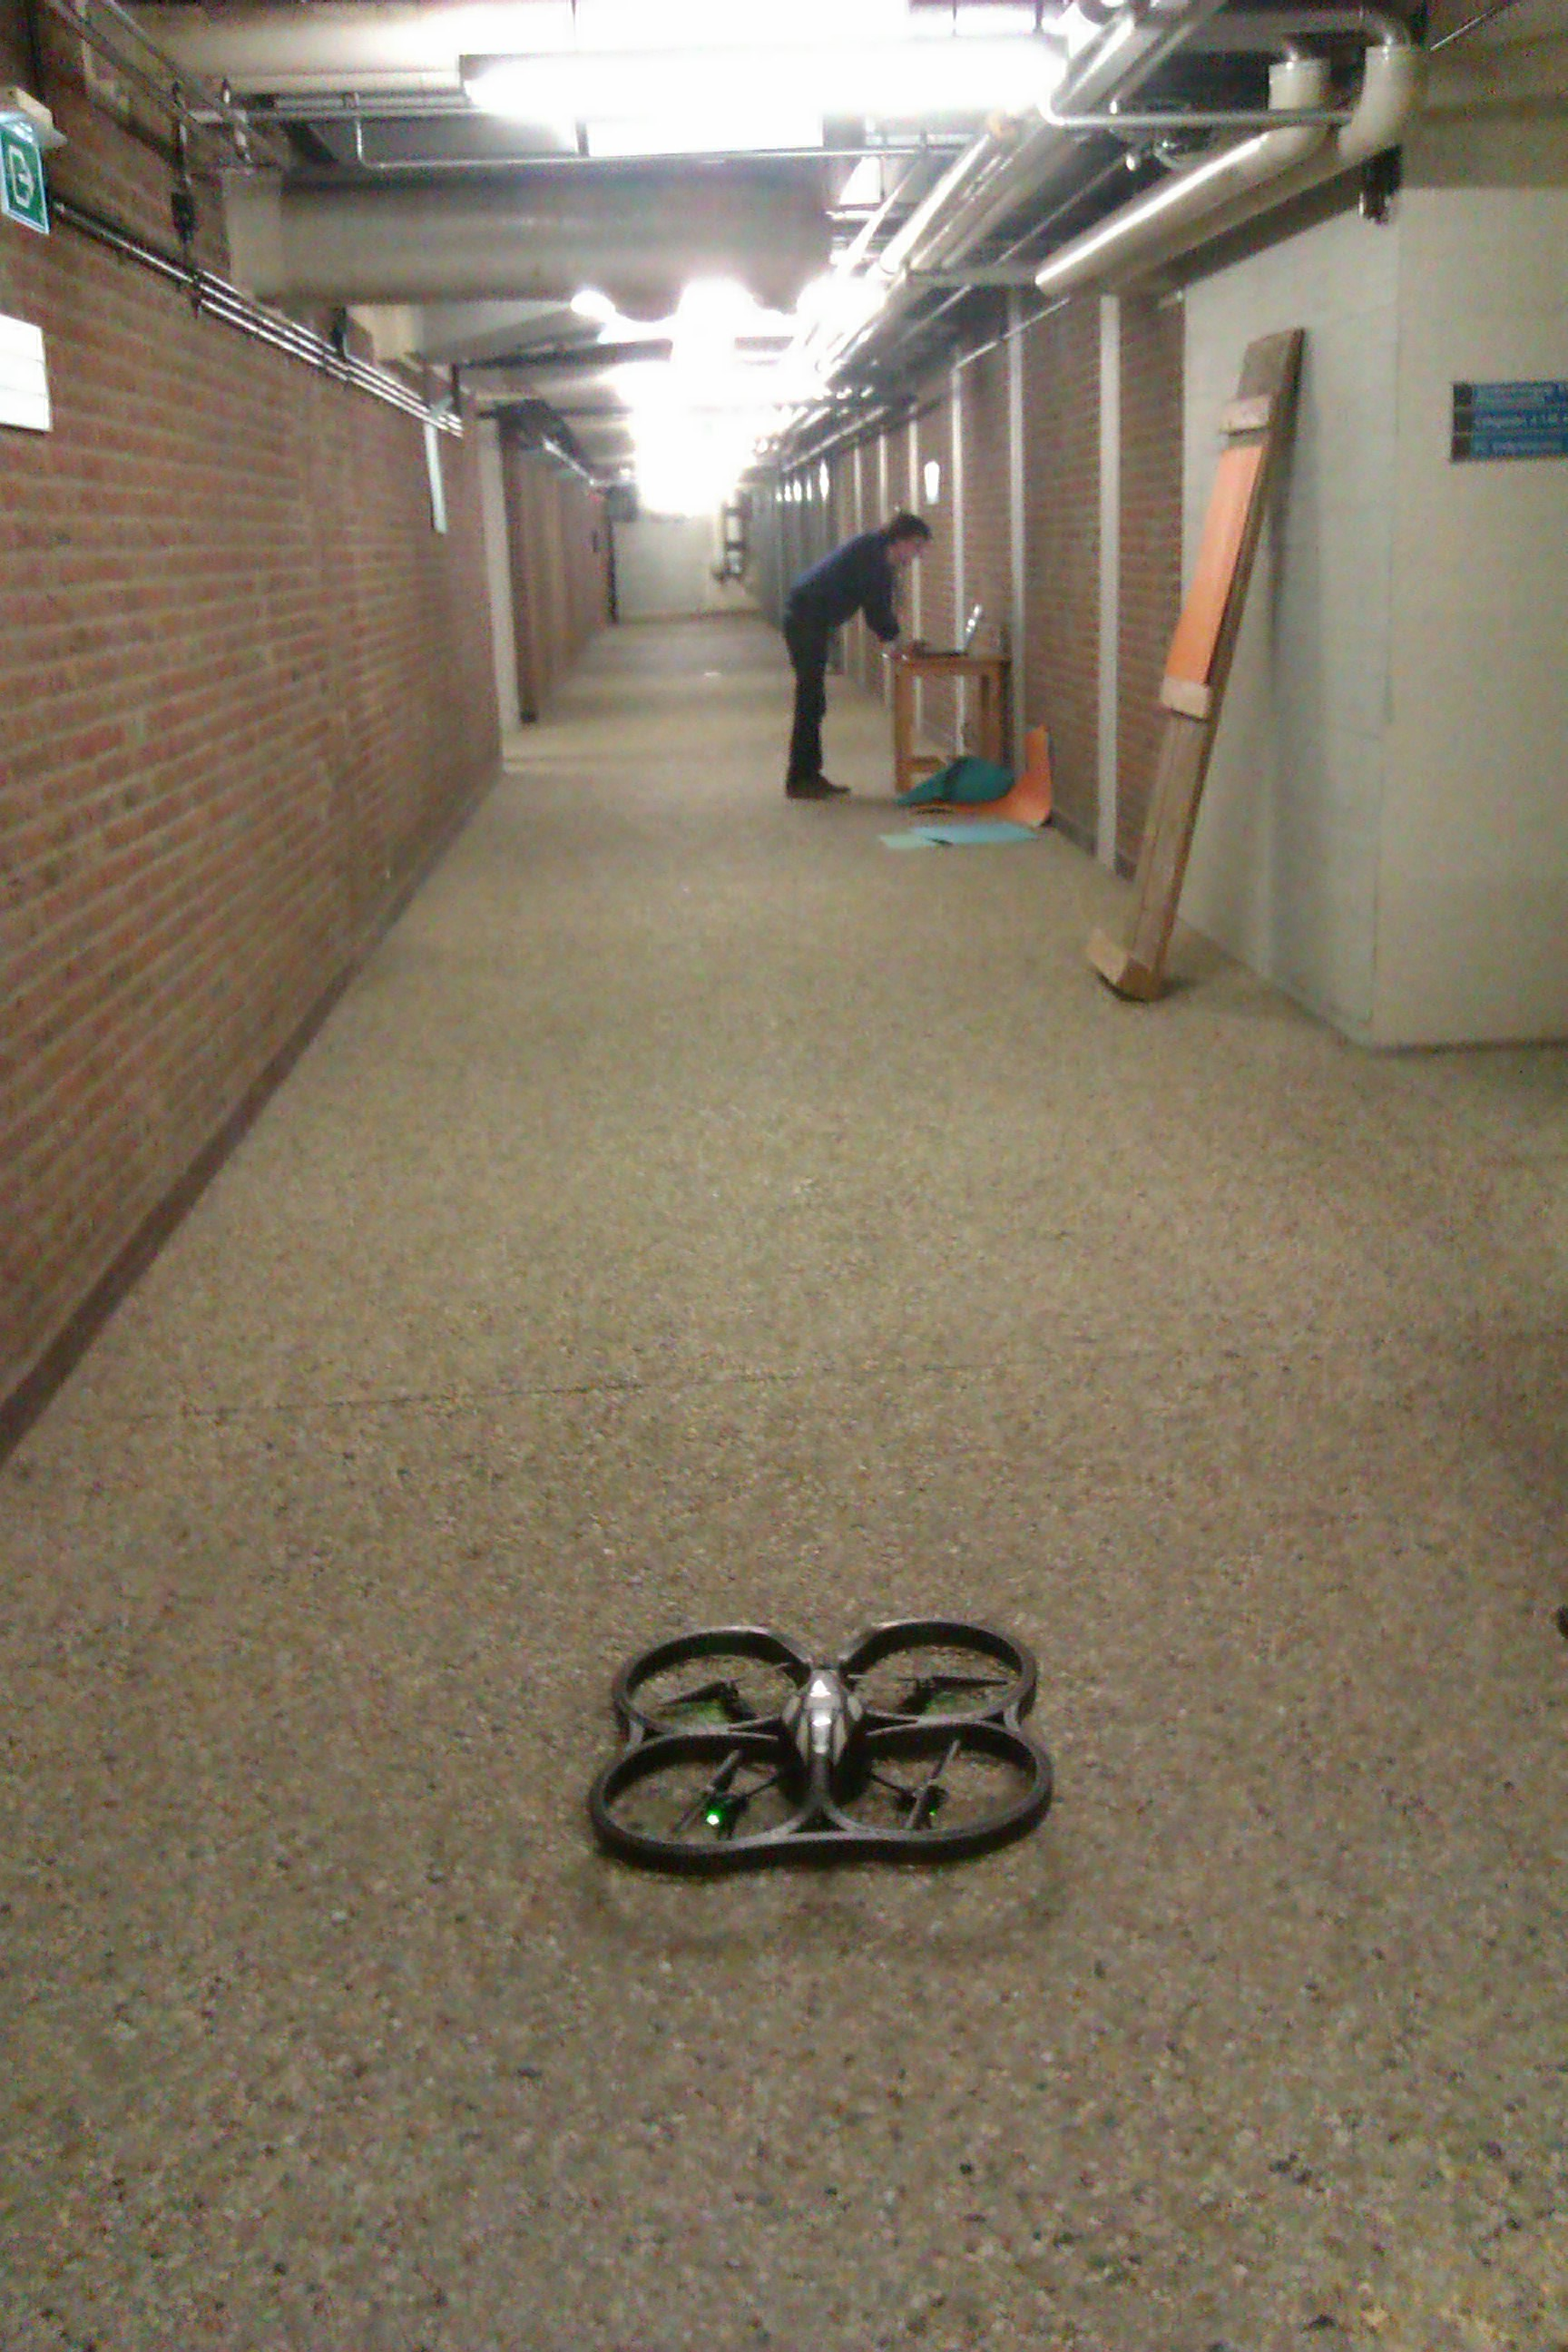
\includegraphics[width=0.5\textwidth]{images/boringHallway}
\end{figure}

In this section several of the implemented algorithms are discussed. Every subsection starts with the code in pseudocode and ends with an explanation of the algorithm. 
\subsection{Detection of objects}
\begin{verbatim}
targets = getAllBlobsThatMatchOurTarget
coolDownHeatMap
activateHeatMap(targets)
if dot in heatmap is high enough
    if sum of heatmap is high enough
        inspect package
    else
        go toward average of activation
\end{verbatim}
Our program first determines that targets we have by acquiring all blobs that match our target.
After this is done our heatmap is cooled down multiplying every activation value by $0.5$. 
The heatmap then receives activation again by raising the value of all the locations of the detected blobs. 
When a dot in our heatmap is activated enough it is assumed that this is because our target is at this position. 
When the total sum of the heatmap is activated enough we "inspect" the package (see section \ref{sec:packageinspection}). 
When there is not enough activation the drone flies towards the average of the activation (see section \ref{flytowards}).



\subsection{Corridor following} 
\label{sec:corridorfollowing}
\begin{verbatim}
targets = getAllBlobsThatMatchOurTarget
myTarget = getTargetLowestOnCamera
if isVeryMuchToTheLeft(myTarget)
    flyVeryHardToTheleft
else if isVeryMuchToTheRight(myTarget)
    flyVeryHardToTheRight
else if isSlightlyToTheLeft(myTarget)
    flySlowlyToTheLeft
else if isSlightlyToTheRight(myTarget)
    flySlowlyToTheRight
else
    flyForward
\end{verbatim}

We found out that by always flying towards the target that was the "lowest" on the camera (in the y-space) our drone could smoothly follow the lights in the hallway. 
By implementing this function we were able to get a corridor-following behaviour. 
Our program first gets all blobs that are matching our target colour (the color of the lights). 
The blob with the lowest y value is chosen as our primary target. 
When this blob is very much to the left or right the drone will turn with a great speed in this direction. 
When this blob is only slightly to the left or right the drone will turn slowly in this direction. 
Otherwise the drone will fly forwards this blob. 

\subsection{Flying towards objects\label{flytowards}}
\begin{verbatim}
direction = XvalueOfAverageOfActivation
turnTowards(direction)
flyForward
\end{verbatim}

Flying towards a target was first solved by only flying towards a specific blob. 
As soon as we started working with objects that were not detected as a "whole" blob and we had an activation value we thought of another function. 
In the new fly-towards function the X value of the average of the activation is taken.
This value is divided by the length of the camera image and mapped to our drone in such a way that we acquire a directional value. 
We let the drone "spin" in this direction and fly forwards. 

\subsection{Package inspection\label{sec:packageinspection}}
\begin{verbatim}
if sum(activation) > threshold
    if getNewTarget(currentTarget)
        currentTarget = getNewTarget(currentTarget)
    else
        startLanding
\end{verbatim}

For the "inspection" of the packages there is not a really special behaviour. 
As soon as the total activation in the heatmap for the packages exceeds the set threshold the next target is chosen. 
When there is no new target specified in our goals-array the drone will land. 

%%%%%%%%%%%%%%%%%%%%%%%%%%%%%%%%%%%%%%%%%%%%%%%%%%%%%%%%%%%%%%%%%%%%%%%%%%%%%%%
% DIVISION OF LABOUR
%%%%%%%%%%%%%%%%%%%%%%%%%%%%%%%%%%%%%%%%%%%%%%%%%%%%%%%%%%%%%%%%%%%%%%%%%%%%%%%
\section{Project history and division of labour}
\label{sec:projecthistory}
The first BioMAV project started in 2010 with an enthusiastic group of people (as described in section \ref{sec:background}). 
After the initial project was a large success and obtained the third price in the IMAV 2011 pylon challenge, a sequel to this project was started.
For this second project one had to write a solicitation letter and send this to the teachers. 
Initially the group consisted of a group of 5 students (Youetta, Rick, Jurriaan, Roland and Robin).  
These people were divided into two teams, the "image processing" team and the "drone control" group. 
The task of the "image processing" team, consisting of Rick, Jurriaan and Robin, was defined as getting useful features from the image data, which would be given to the "drone control" group.
The "drone control" group, consisting of Roland and Youetta, was supposed to use these features to control the drone. 


Initially both groups were both trying to decode the largely undocumented code made by the previous team.
One of the wishes of the group was a code implementation using ROS, this was another software part that both teams had to figure out how to use. 
Around June the first implementation of a control program using ROS was finished by Roland. 
This program consisted of a server extension of the original software written by the first BioMAV team.  
The ROS component connected to a socket that listened to calls coming from the ROS component of the software. 
Using a simple syntax to parse fly-commands it was possible to fly with the ARDrone using ROS.  

Unfortunately, other team members turned out to be not that enthusiastic about the project anymore. 
Some stopped pretty early and told the whole group about it, others stopped very late without telling anybody.
This all led to the fact that the project slowed down and was not really coordinated anymore. 

During a meeting in July it was agreed that this setup was not useful enough and that another implementation had to be found that only used ROS. 
Unfortunately this meant that Robin and Roland had to start over again, throwing away all old code (including all code produced by the first BioMAV project).  
After we threw away all old code we started with searching this "easy usable" library that should have been available on the internet. 
Unfortunately, this did cost us more time than we expected.
Every library we found was either not usable, not downloadable (findable) anymore or not uploaded yet (but sounded very promising). 
It was only after a lot of hours searching that one of the libraries suddenly was pullable again. 

After we were able to control the drone using this library we started looking at how we would be able to recognise objects. 
We started with looking at the recognition of colours, which thanks to a remark by Bas Bootsma turned out to be relatively simple. 
His idea was to recognize blobs using the cmvision library \cite{cmvision}. 
Starting this library turned out to be pretty easy, tweaking it turned out to cost more time than expected. 

Although recognizing blobs worked for recognizing objects it also yielded a lot of "false-positives", objects that did not have to be recognized.
As an alternative we started to look at alternatives, including using AR markers and image-recognition. 
Unfortunately it proved to be too much of a challenge to use the algorithms available on ROS with the image data that we acquired. 

Unfortunately this did not solve our problem about recognizing objects that were not our target as target objects.
The first solution we came up with was searching for the most dull location, this turned out to be the corridor under the Spinoza building. 
Although this hallway did not contain a lot of colours and distractions from our real target there were still a lot of small blobs recognised by our blob-detector. 

Our first solution was to simply ignore small blobs and try to use colours that were more different than those colours found in the hallway. 
This did lead to a more stable blob recognition, but still was not perfect. 

The small blobs scattered a lot while the blob of our real object was pretty stable. 
Eventually we came up with the idea to use a "heat-map", where all detected blobs would yield an activation. 
Over the course of several frames this activation would decay leading to the fact that only locations where for longer times blobs were detected would be activated. 

This led to a very smooth detection of the target object, as is visible in figure \ref{fig:robinPresentActivation}. 

\begin{figure}[h!]
	\caption{Robin with a target in the left image, on the right is the activation}
	\centering
	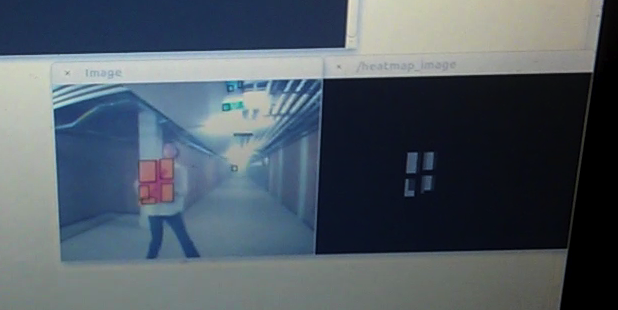
\includegraphics[width=0.5\textwidth]{images/robinPresentActivation}
	\label{fig:robinPresentActivation}
\end{figure}

\begin{figure}[h!]
	\caption{A picture of a drone.}
	\centering
	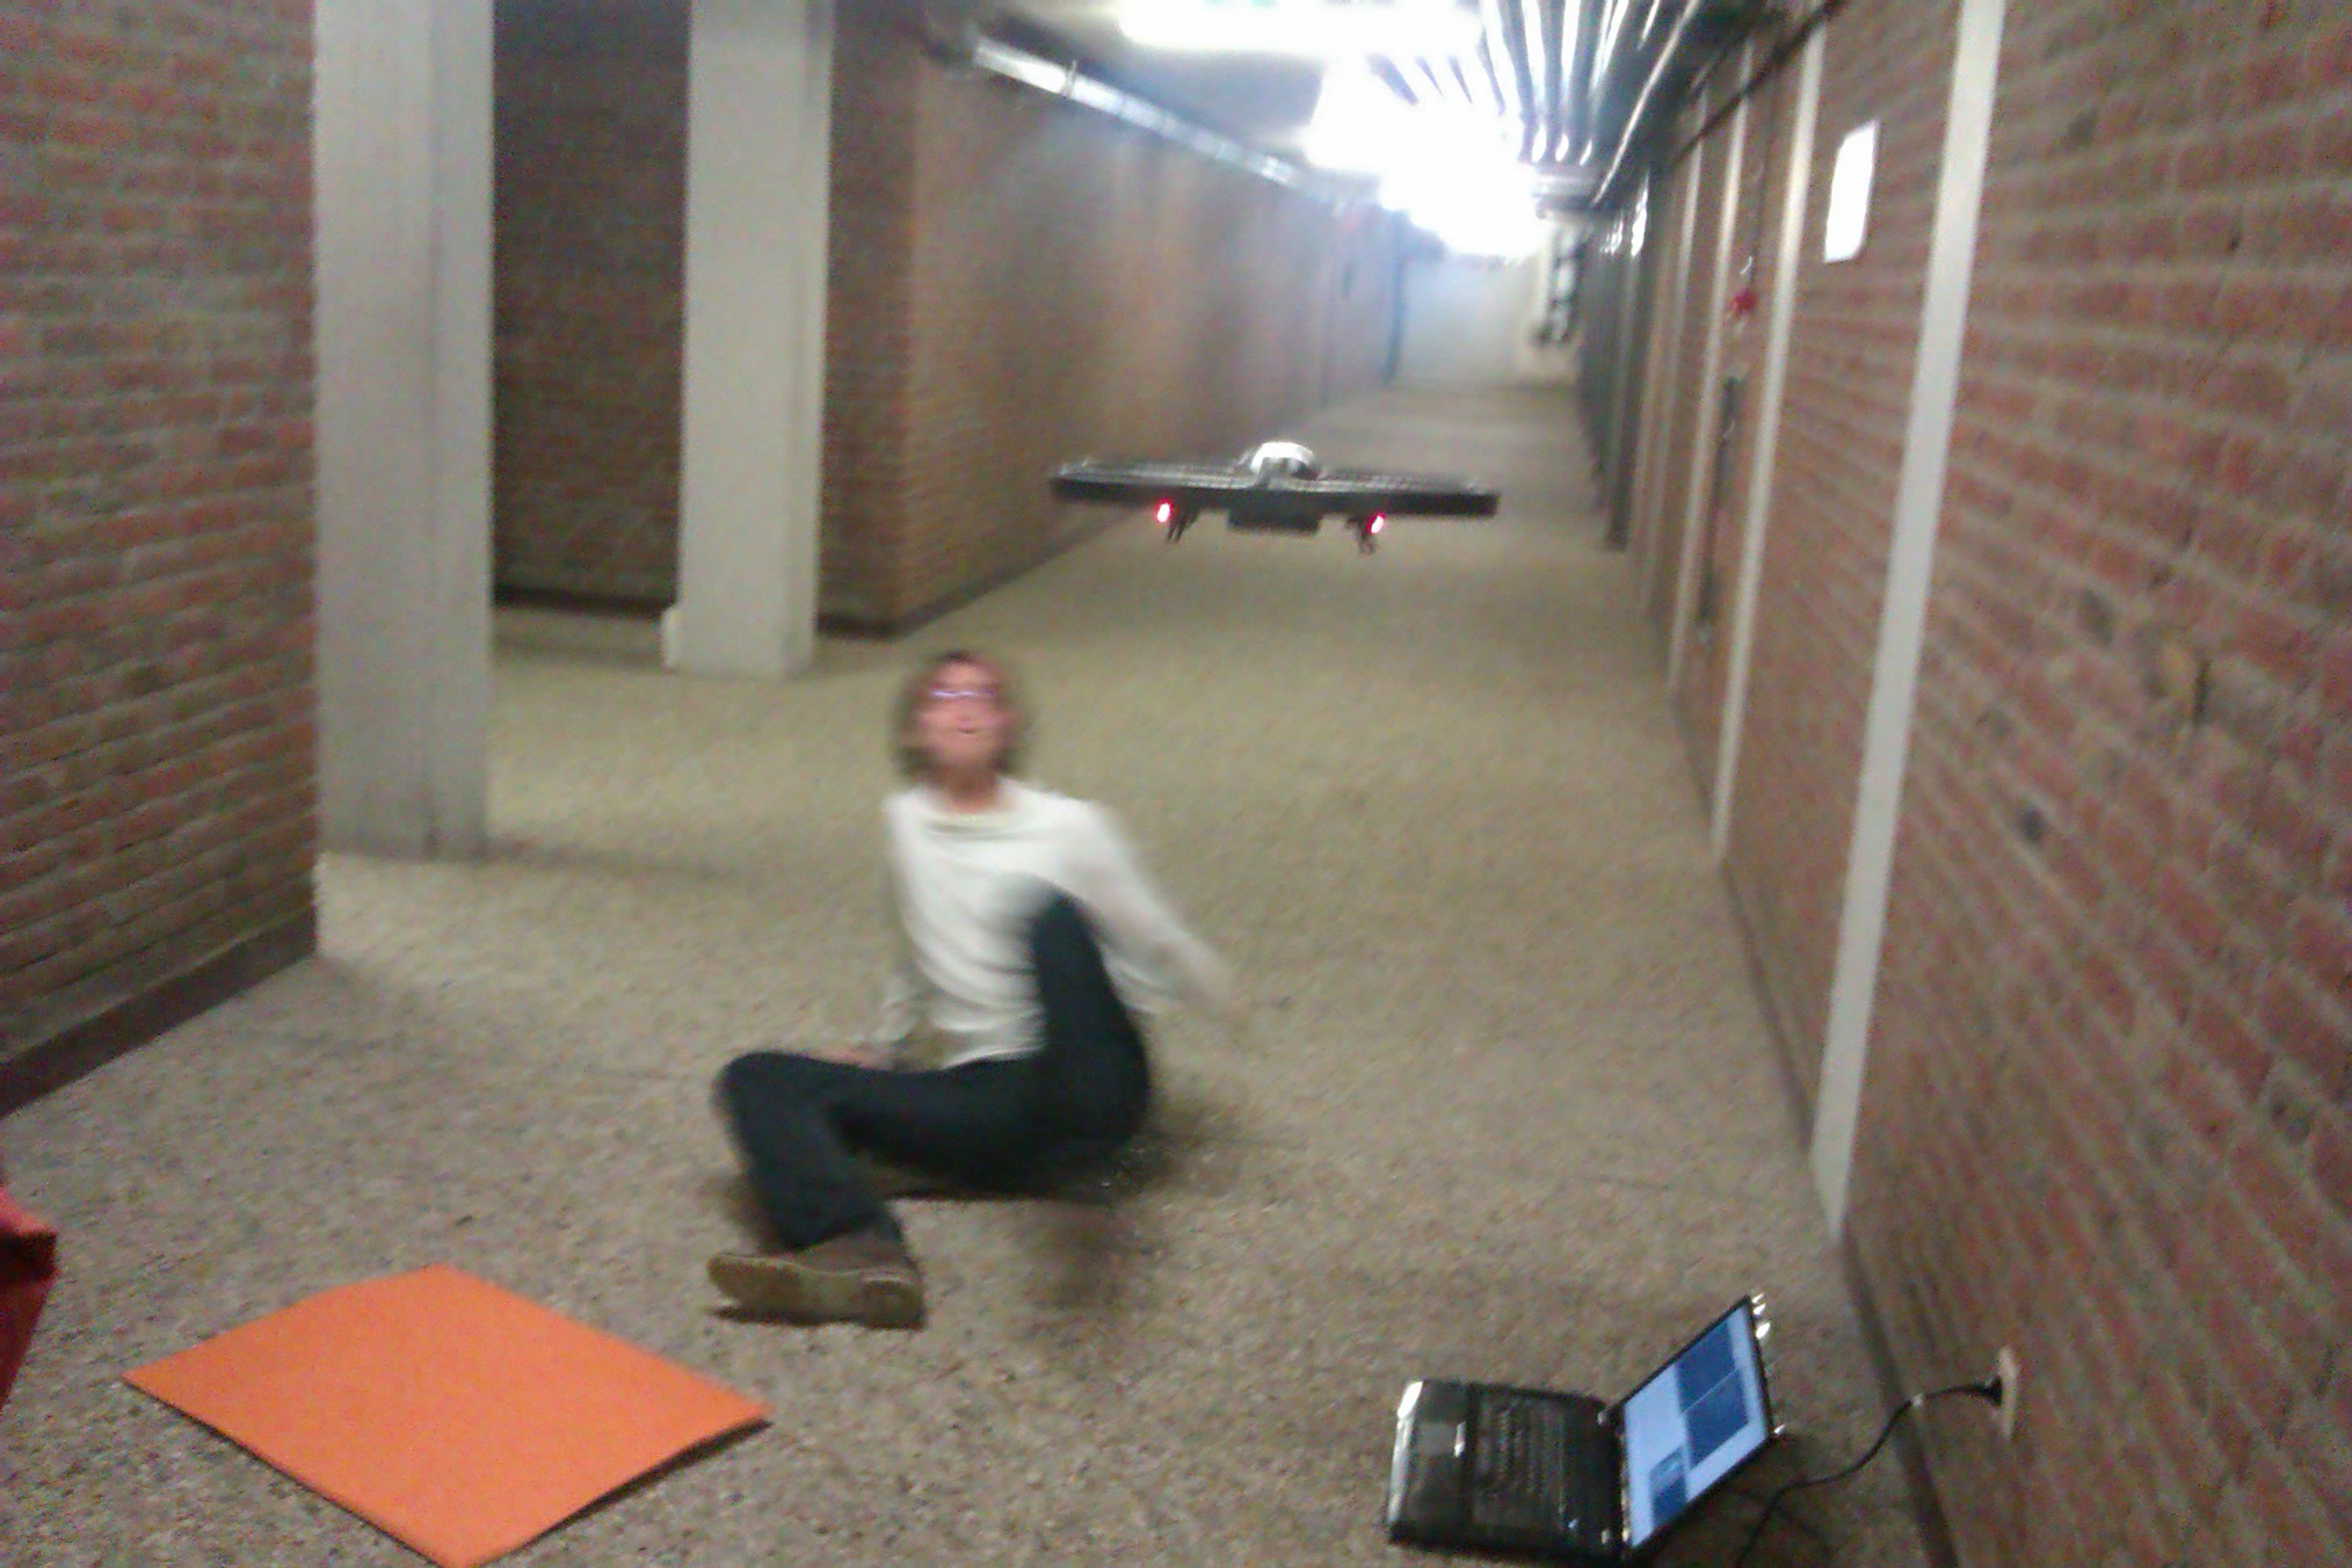
\includegraphics[width=0.5\textwidth]{images/droneAttack}
\end{figure}

%%%%%%%%%%%%%%%%%%%%%%%%%%%%%%%%%%%%%%%%%%%%%%%%%%%%%%%%%%%%%%%%%%%%%%%%%%%%%%%
% TUTORIAL
%%%%%%%%%%%%%%%%%%%%%%%%%%%%%%%%%%%%%%%%%%%%%%%%%%%%%%%%%%%%%%%%%%%%%%%%%%%%%%%
\section{Tutorial}
\subsection{Installation}
To install ROSMAV, follow the following steps:
\begin{enumerate}
\item Install Ubuntu (we used Ubuntu 10.10).

\item Install ROS (we used Electric) by following this guide: \\
      http://www.ros.org/wiki/electric/Installation/Ubuntu

\item Make sure that you performed the ``Environment setup'' step during installation.

\item Download our repository from
      https://github.com/dutchcheesehead/ROSMAV

\item Navigate to ROSMAV.

\item Run \textbf{./install.sh}.
\end{enumerate}

\subsection{Starting ROSMAV}
To start our software, run the following commands all in different terminal windows:
\begin{enumerate}
\item \textbf{roscore} \\ This starts roscore.
\item \textbf{rosrun ardrone\_brown ardrone\_driver} \\ This starts the driver for the AR-Drone.
\item \textbf{roslaunch cmvision blobs.launch} \\ This starts the blob detection process.
\item \textbf{brown-ros-pkg-read-only/experimental/drone\_teleop/bin/drone\_teleop.py} \\ This is needed to let the drone take off and land.
\item \textbf{rosrun image\_view image\_view image:=/heatmap\_image} \\ This
      allows you to see the heatmap activation for the ``inspect presents''
      task, and thus see through the eyes of the drone.
\item \textbf{rosrun ROSMAV inspectPresents.py} \textit{or} \\
      \textbf{rosrun ROSMAV followLights.py} \\
      This actually starts the task. 
\end{enumerate}
\subsection{Adding different colors to inspect}
Suppose you want to add a different color to inspect.
\begin{enumerate}
\item Run \textbf{roscore}
\item In another terminal window, start the AR-Drone driver: \textbf{rosrun ardrone\_brown ardrone\_driver}
\item Start the ColorGUI: \textbf{rosrun cmvision colorgui image:=/ardrone/image\_raw} \\
      You will see a window with the camera images from the AR-Drone.
\item Resize the window so you can see the text fields.
\item Keep the object you want to inspect in the view of the drone.
\item Click on the image of that object in the ColorGUI on a few different places.
\item Move both the object and the drone a bit around and click some more, to account for changes in lighting.
\item Repeat until you are confident it recognizes the object correctly in different circumstances.
\item If you made a mistake, close the ColorGUI and go back to step 3.
\item If it recognizes the object correctly, open ``cmvision/colors.txt''. Add both the color and the threshold. For the color, you can copy the last color and change the first bit into what the ColorGUI said, and change the name of the color. For the threshold, paste the threshold after the last threshold.
\item Edit ``inspectPresents.py''. You might need to add a function like ``isRed'' if it's not already in there. Then modify the ``nextTarget'' dictionary to the sequence you want to inspect the presents.
\end{enumerate}

%%%%%%%%%%%%%%%%%%%%%%%%%%%%%%%%%%%%%%%%%%%%%%%%%%%%%%%%%%%%%%%%%%%%%%%%%%%%%%%
% REFLECTION
%%%%%%%%%%%%%%%%%%%%%%%%%%%%%%%%%%%%%%%%%%%%%%%%%%%%%%%%%%%%%%%%%%%%%%%%%%%%%%%
\section{Reflection}
\label{sec:reflection}

Although the BioMAV project has been a rough project this year the final result is something that looks very cool. 
To build a program that lets a small UAV autonomously follow bread-containers, corridors and inspect packages is something to be proud of. 

Of course, one starts to think about how much more awesome the initial plans of the complete team were. 
Unfortunately, since more than half of the team decided to stop early, these plans were never finished and kept for the next team. 

Another thing that was very unfortunate was the fact that the whole old BioMAV project was thrown away in the end. 
Although a lot of time was spend in learning how to interpret the old code and extending the project to work with ROS all these work was thrown away. 
Another thing that was not used after a lot of time went into researching this were the AR markers, unfortunately these proved to be impossible for us to implement. 

Of course we are all very contend with the final result, and are very proud about what we eventually reached in such a short time. 

\begin{figure}[h!]
	\caption{A picture of a drone.}
	\centering
	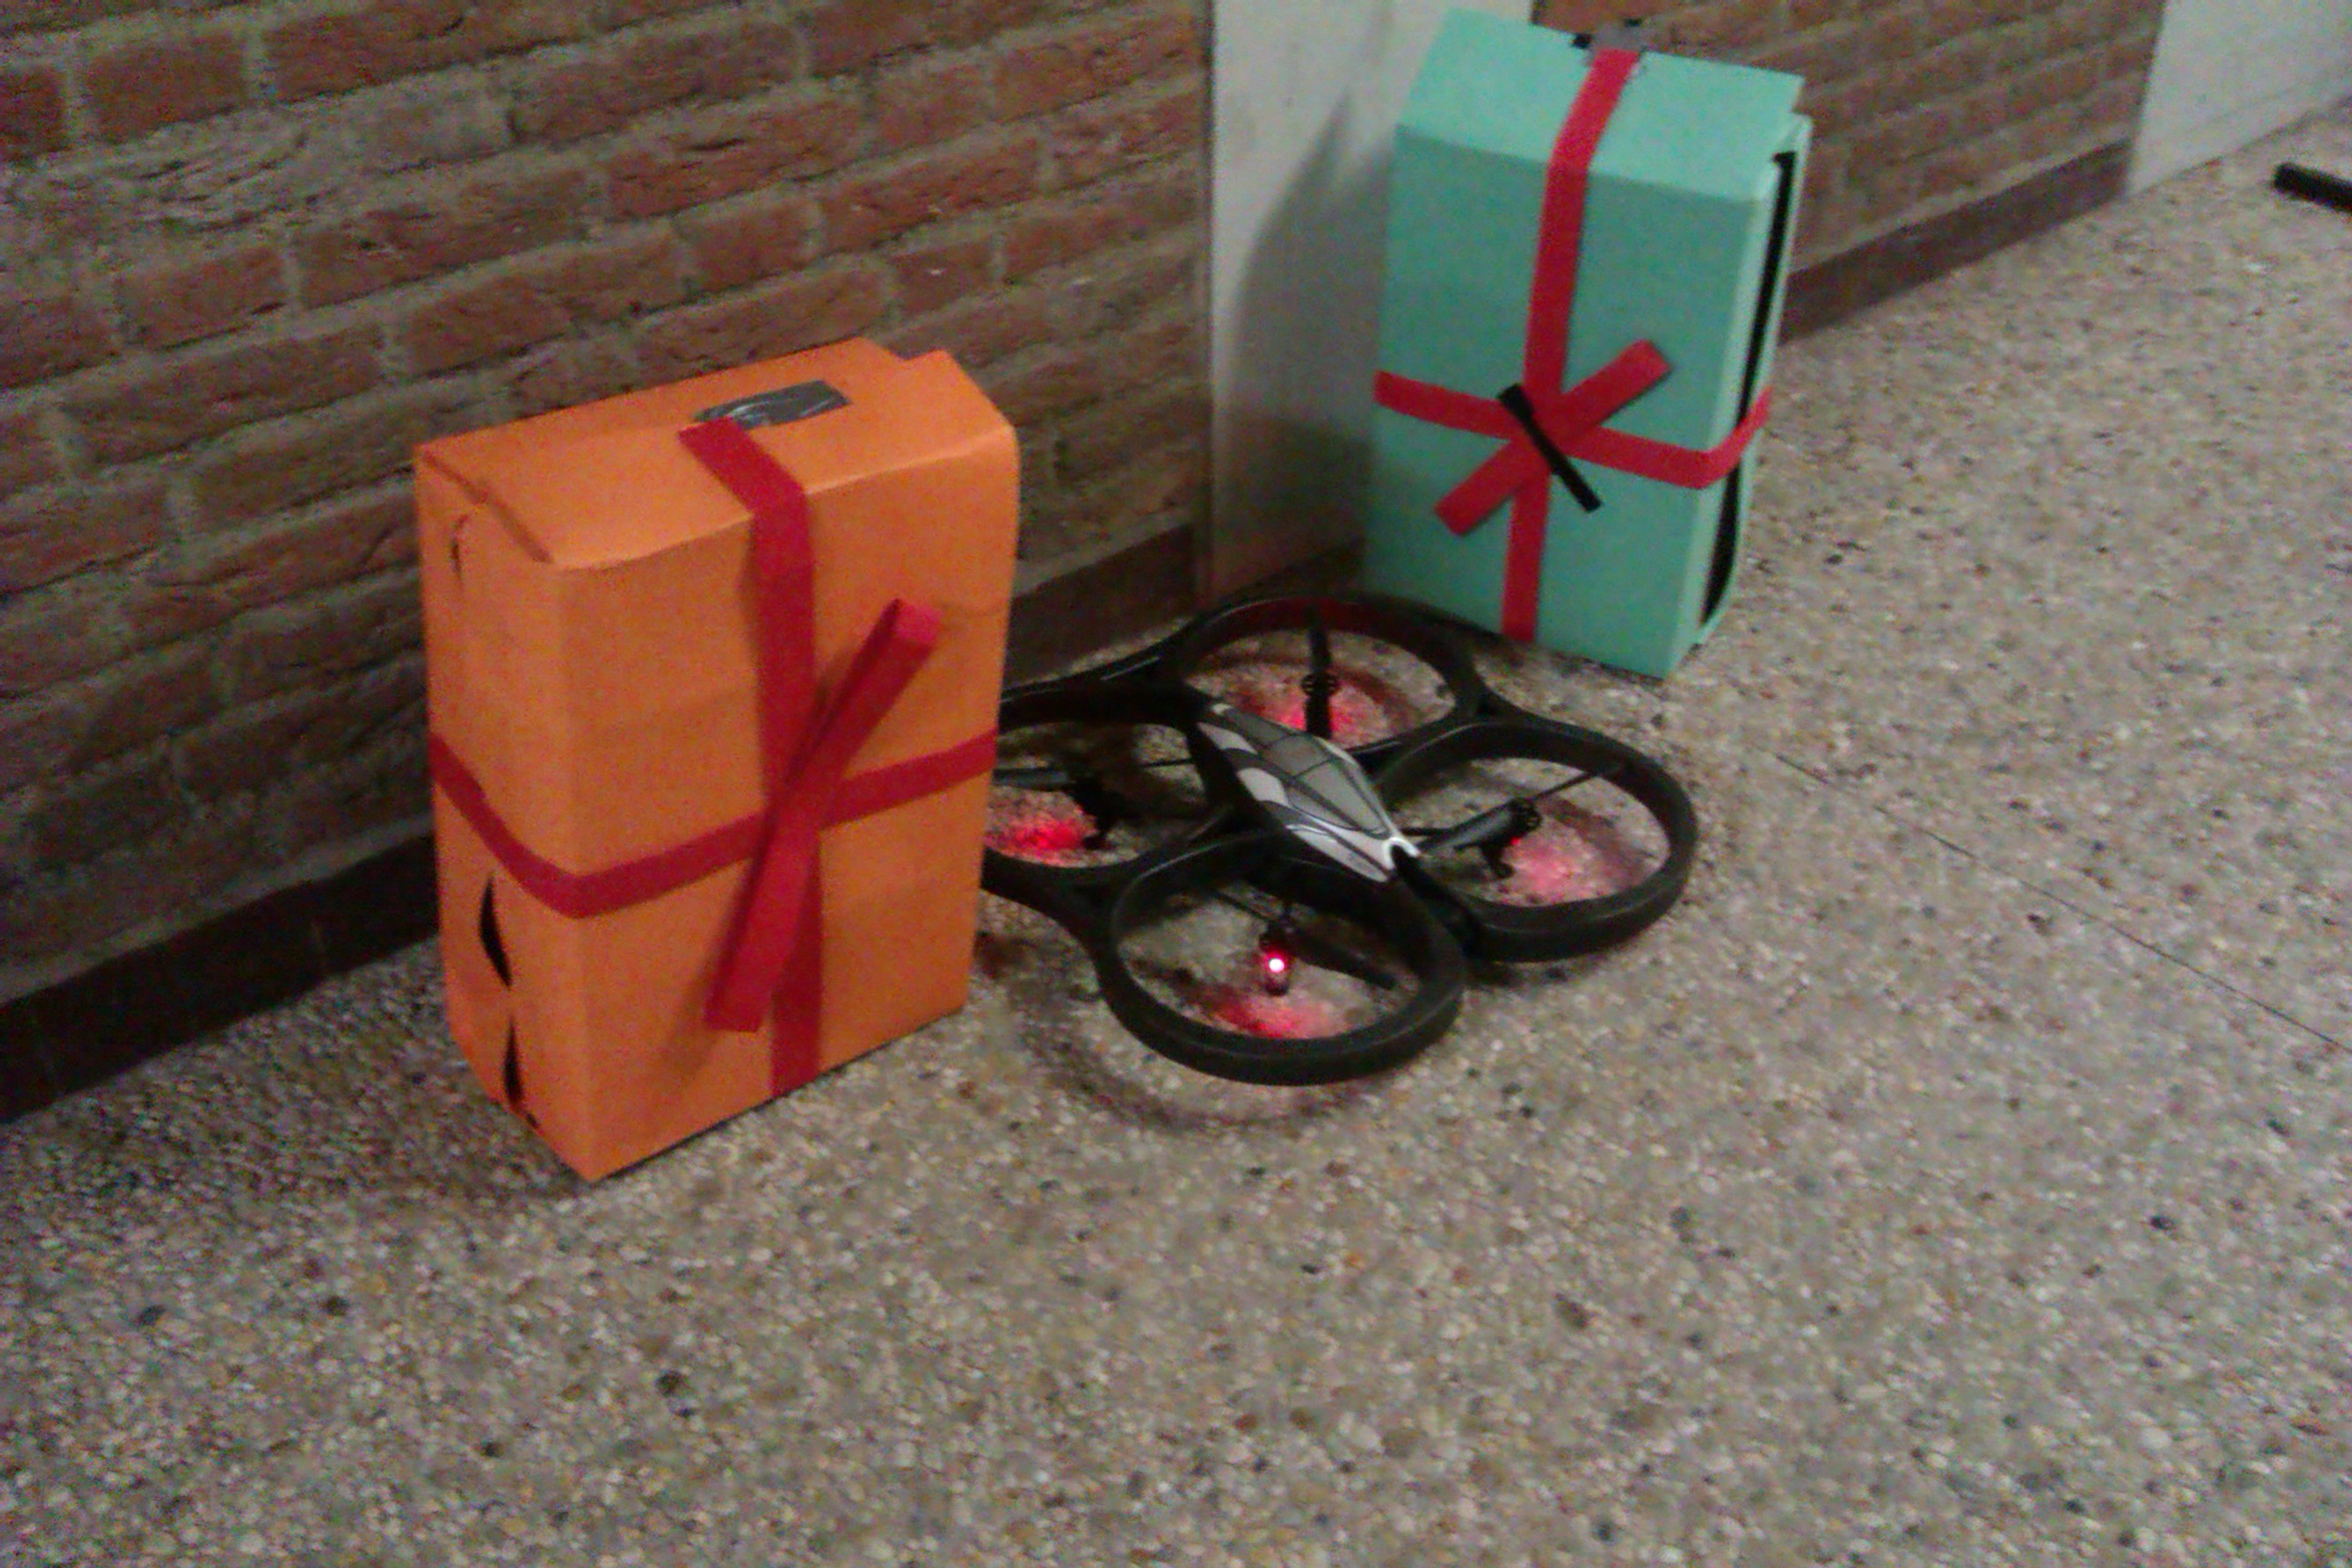
\includegraphics[width=0.5\textwidth]{images/presentsAndDrone}
\end{figure}
%%%%%%%%%%%%%%%%%%%%%%%%%%%%%%%%%%%%%%%%%%%%%%%%%%%%%%%%%%%%%%%%%%%%%%%%%%%%%%%
% BIBLIOGRAPHY
%%%%%%%%%%%%%%%%%%%%%%%%%%%%%%%%%%%%%%%%%%%%%%%%%%%%%%%%%%%%%%%%%%%%%%%%%%%%%%%
\bibliographystyle{plain}
\bibliography{bibliography}

\end{document}
